\documentclass[12pt, french]{article}

\usepackage{fancyhdr, fancybox, lastpage,mhchem, mathrsfs}
\usepackage[most]{tcolorbox}
\usepackage[a4paper, margin={0.3in, .75in}]{geometry}
\usepackage{wrapfig}
\pagestyle{fancy}
\renewcommand\headrulewidth{1pt}
\renewcommand\footrulewidth{1pt}
\fancyhf{}
\rhead{ \em{Zakaria Haouzan}}
\lhead[C]{\em{2ème année baccalauréat Sciences Physiques}}
\chead[C]{}
\rfoot[C]{}
\lfoot[R]{}
\cfoot[]{\em{Page \thepage / \pageref{LastPage}}}


\newtcolorbox{Box2}[2][
enhanced, 
    breakable,
]{
                lower separated=false,
                colback=white,
colframe=white!20!black,fonttitle=\bfseries,
colbacktitle=white!30!gray,
coltitle=black,
enhanced,
attach boxed title to top left={yshift=-0.1in,xshift=0.15in},
title=#2,#1}


\begin{document}
\begin{center}
   \shadowbox {\bf{Exemples des transformations forcées: l'électrolyse}
 }

\end{center}

\vspace{-0.2cm}
%%_________________________Exercice ! :"_________________________Exercice
   \begin{Box2}{Exercice 1 : gaz d'une grande pureté.}
	   \begin{wrapfigure}[5]{r}{0.42\textwidth}
  \begin{center}
	  \vspace{-0.6cm}
	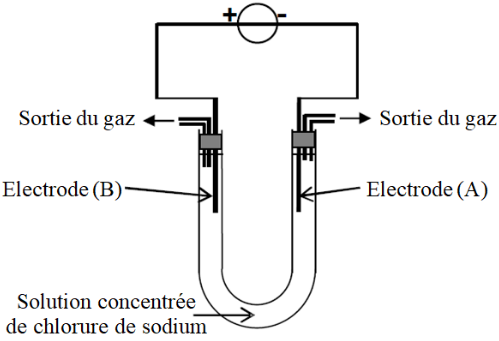
\includegraphics[width=0.42\textwidth]{./ex00.png}
  \end{center}
\end{wrapfigure}
	   \emph{L'électrolyse permet d'obtenir des gaz d'une grande pureté.
On réalise l'électrolyse d'une solution concentrée de chlorure de sodium
$Na^+_{(aq)} + Cl^-_{(aq)}$, on obtient un dégagement de dichlore au voisinage de l’une des
électrodes, et dégagement de dihydrogène au voisinage de l'autre électrode, de plus
que le milieu réactionnel \\devient basique au cours de la transformation chimique.}

\begin{itemize}
	\item Les couples intervenants dans la transformation\\ chimique : $(H_2O_{(l)})/H_{(g)})$ et $(Cl_{2(g)}/Cl^-_{(aq)})$
	\item Le faraday $\mathscr{F}=9,65.10^4 C.mol^{-1}$
	\item Le volume molaire dans les conditions de l’expérience :$V_m = 25,0L.mol^{-1}$
\end{itemize}
La figure ci-contre représente le
dispositif expérimental utilisé pour
réaliser cette électrolyse.

\begin{enumerate}
	\item Déterminer laquelle parmi les
électrodes (A) et (B) celle qui
joue le rôle de l'anode et celle
qui joue le rôle de la cathode.

\item Ecrire l’équation de la réaction
ayant lieu au voisinage de
chaque électrode, et l'équation
bilan de cette électrolyse.

\item Le générateur alimente le circuit avec un courant électrique d'intensité constante
	$I = 3A$. Calculer le volume du dichlore formé pendant la durée $\Delta{t} = 25 min$.
\end{enumerate}


   \end{Box2}


%%_________________________Exercice !2 :"_________________________Exercice
\begin{Box2}{Exercice 2 :La galvanisation }
	\begin{wrapfigure}[6]{r}{0.32\textwidth}
  \begin{center}
	  \vspace{-0.6cm}
	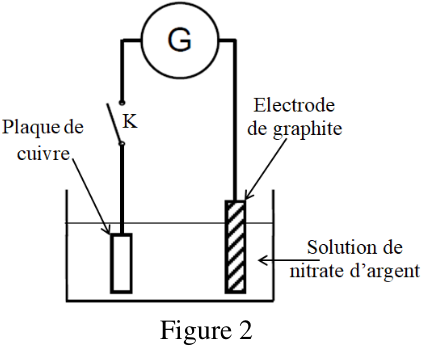
\includegraphics[width=0.32\textwidth]{./ex_01.png}
  \end{center}
\end{wrapfigure}
	\emph{La galvanisation est l’une des applications industrielles de l’électrolyse, visant à
recouvrir un métal par une couche fine d’un autre métal, dans un but de protection
ou d’esthétique.}

Le but de cet exercice est l’étude de l’opération d’argenture d’une pièce de cuivre à
l’aide de l’électrolyse.

\begin{itemize}
	\item Les couples intervenants : $(O_{2(g)}/H_2O_{(l)})$ et $(Ag^+_{(aq)}/Ag_{(s)}$
		
	\item Le faraday:  1$\mathscr{F}=96500 C.mol^{-1}$
	\item La masse molaire atomique de l’argent : $M(Ag) = 108 g.mol^{-1}$
\end{itemize}

On immerge complétement une plaque de cuivre dans une solution (S) de nitrate d'argent $(Ag^+_{(aq)}$+$NO^-_{3(aq)})$ de  concentration molaire C et de volume $V = 0,5 L$.

On relie la plaque par un fil conducteur à
l’un des pôles d’un générateur électrique G,
dont l’autre pôle est relié à une électrode en
graphite (Figure 2). Après la fermeture de
l’interrupteur K, le générateur G alimente,
pendant $\Delta{t} = 45 min$, le circuit par un courant
d’intensité constante $I = 0,5 A$.

On obtient un dégagement du dioxygène $O_2$
au voisinage de l’électrode de graphite et
dépôt d’argent de façon uniforme sur l’autre
électrode.

\begin{enumerate}
	\item Ecrire la demi-équation modélisant la transformation ayant lieu au voisinage de
chaque électrode.
\item Trouver l’expression de la masse m(Ag) d’argent formé en fonction de : I, $\Delta{t}$,
	$M(Ag)$ et $\mathscr{F}$. Calculer sa valeur.
\item  On dispose de deux solutions (S1) et (S2) de nitrate d’argent, de concentrations respectives $C_1 = 1,8.10^{-2} mol.L^{-1}$ et $C_2 = 3.10^{-2} mol.L^{-1}$ et de même volume
$V = 0,5 L$.
Déterminer parmi ces deux solutions celle qui permet d’obtenir la masse m(Ag).
\end{enumerate}

\end{Box2}

%\vspace{-0.8cm}
\begin{center}
   \Large{ \em{Exercices Supplémentaires}}
\end{center}

%\vspace{-0.8cm}

%%_________________________Exercice ! 3:"_________________________Exercice
\begin{Box2}{Exercice 3 : La synthèse de quelques métaux}
%\begin{wrapfigure}{r}{0.4\textwidth}
  %\begin{center}
	%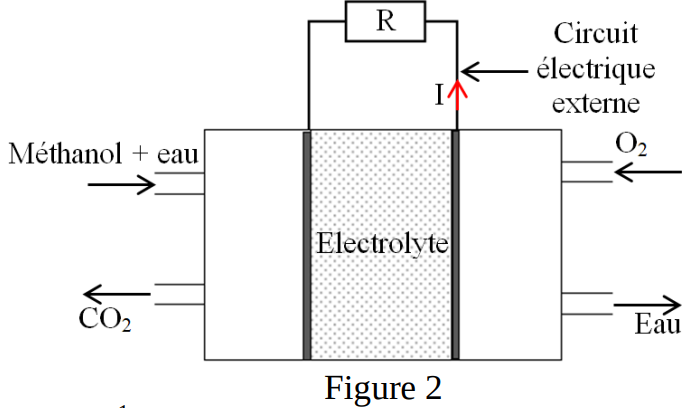
\includegraphics[width=0.4\textwidth]{./ex02.png}
  %\end{center}
%\end{wrapfigure}
	\emph{L’électrolyse est l’une des principales téchniques adoptées aux laboratoires ou dans
les domaines industrièls. elle permet la synthèse de quelques métaux, et d’autres
composés chimiques utilisés dans la vie quotidienne.}

Le but de cette partie de l’exercice est la synthèse du dibrome $Br_2$ et du métal cuivre
par électrolyse.

La masse molaire du cuivre : $M(Cu) = 63,5 g.mol^{-1}$


On réalise l’électrolyse d’une solution de bromure de cuivre II de formule $(Cu^{2+}_{(aq)}+2.Br^-_{(aq)})$ en utilisant deux électrodes $E_1$ et $E_2$ en graphite, il se forme ainsi du
dibrome $Br_{2(l)}$ au voisinage de $E_1$ et dépôt de cuivre au voisinage de $E_2$.

\begin{enumerate}
	\item  Représenter le dispositif expérimental de cette électrolyse, en précisant la
cathode et l’anode.
\item  Ecrire la demie équation modélisant la réaction ayant lieu au voisinage de
chaque électrode.
\item  En déduire l’équation bilan modélisant la transformation ayant lieu au cours de
l’électrolyse.
\item Un générateur alimente le circuit électrique par un courant d’intensité constante
	$I = 0,5 A$ pendant une durée $\Delta{t} = 2 h$.
Déterminer la masse m du cuivre produit au cours de la durée de fonctionnement
de l’électrolyseur.
\end{enumerate}
\end{Box2}

%%_________________________Exercice 4 : _________________________Exercice
\begin{Box2}{Exercice 4 : }
   % \begin{wrapfigure}[12]{r}{0.5\textwidth}
  %\begin{center}
	  %\vspace{-0.6cm}
	%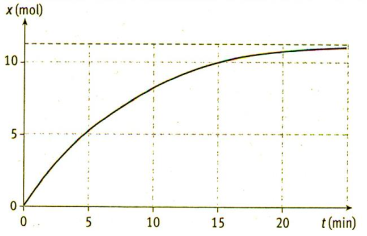
\includegraphics[width=0.5\textwidth]{./img/ex4.png}
  %\end{center}
%\end{wrapfigure}
	Volume molaire des gaz dans les conditions de l’expérience : $V_m = 24 L.mol^{-1}.$
	On réalise l’électrolyse d’une solution de chlorure d’étain II de formule $(Sn^{2+}_{(aq)} + 2Cl^-_{(aq)})$ , en utilisant deux électrodes en graphite. On observe la formation du
	dichlore gazeux  $Cl_{2(l)}$ au voisinage de l’une des électrodes, et un dépôt métallique
	d’étain $Sn_{(S)}$ sur l’autre électrode.
	\begin{enumerate}
		\item  Représenter le dispositif expérimental de cette électrolyse, en précisant la
cathode et l’anode.
\item  Ecrire l’équation modélisant la réaction ayant lieu au voisinage de chaque
électrode et en déduire l’équation bilan modélisant la transformation ayant lieu
au cours de l’électrolyse.
\item  Un générateur alimente le circuit électrique par un courant d’intensité constante
	I = 1,5 A pendant une durée $\Delta{t} = 80 min$.
Déterminer le volume du dichlore produit au cours de la durée de
fonctionnement de l’électrolyseur.
\end{enumerate}
\end{Box2}

\begin{center}
	\emph{\textbf{Don't trust, check!}}
\end{center}

%\vspace{-0.6cm}
%%%_________________________Exercice 5 : _________________________Exercice
%\begin{Box2}{Exercice 4 : }
   %% \begin{wrapfigure}[14]{r}{0.5\textwidth}
  %%\begin{center}
	  %%\vspace{-0.6cm}
	%%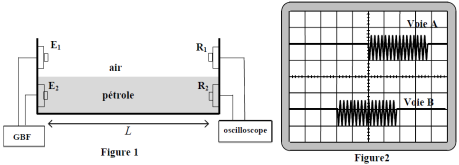
\includegraphics[width=0.5\textwidth]{./img/ex5.png}
  %%\end{center}
%%\end{wrapfigure}

%4

%\end{Box2}

%\begin{Box2}{Exercice 5 : }

%44
%\end{Box2}


%\begin{Box2}{Exercice 6 : }


	%\end{Box2}


%\begin{Box2}{Exercice 7 : }
%\end{Box2}
\end{document}
